\section{The Advanced Encryption Standard (AES)}

On September 12, 1997, the United States' National Institute of
Standards and Technology (NIST) announced an open competition to
develop a new symmetric-key block cipher algorithm to replace the
ageing DES (Data Encryption Standard). The demands was that the AES
should be an unclassified, public, and royalty-free symmetric-key
encryption algorithm supporting block sizes of 128-bits, key sizes of
128-, 192- and 256-bits.

On October 2, 2000, NIST announced that it had selected
Rijandael~\cite{rijandael}, designed by two Belgium cryptographers:
Daemen and Rijmen, as the AES.

%As of today, multiple processors include native support for
%acceleration of AES-specific operations. NIST has also called for the
%development of a new hash-function, and 4 of 14 of the remaining
%candidates rely on native AES-acceleration to acheive performance.

\subsection{Overview of the algorithm}

Rijandael is a symmetric-key block-cipher algorithm. This means that
encryption is defined as $c \leftarrow E_k(m)$, and decryption as $m
\leftarrow D_k(c)$, given a key $k$, a message $m$ and a ciphertext
$c$. Rijandael supports variable block and key sizes, but I will
confine the description and implementation to block and key size to
128~bits. This will not cause a big loss of generality to the working
principle. I will also limit the implementation to encryption-only.

The Rijandael cipher segments a 128-bit message into 16 bytes,
represented by a $4 \times 4$ matrix:

\begin{equation}
  m = \begin{pmatrix}
    m_0 & m_4 & m_8 & m_{12} \\
    m_1 & m_5 & m_9 & m_{13} \\
    m_2 & m_6 & m_{10} & m_{14} \\
    m_3 & m_7 & m_{11} & m_{15}
    \end{pmatrix}
\end{equation}

This is referred to as the $State$ througout the algorithm, and it
is permutated 10 rounds in the algorithm. For larger key sizes, the
number of rounds should be increased. A round is composed of four
transformations described below:

\begin{eqnarray*}
&Round&(State, RoundKey) \{\\
  & &SubBytes (State)\\
  & &ShiftRows (State)\\
  & &MixColumns (State)\\
  & &AddRoundKey (State, RoundKey)\\
&\}&
\end{eqnarray*}

The final round, $FinalRound$, is slightly different: it excludes the
MixColumns stage. $RoundKey$ is derived from the key by the key
expansion scheme also described below. For decrypting, given the
correct key, there exists inverse functions for each round.

The Rijandael cipher work in a finite field. The field is realized as
all polynomials modulo the irreducivle polynomial $f(x) = x^8 + x^4 +
x^3 + x + 1$ over $\mathbb{F}_2$. This is called the ``Rijandael
field'', and $\mathbb{F}_{2^8}$ is often used to denote the field with
256 element. Each element can also be represented as a 8-bit byte. All
operations on elements in this field results in an element within the
field. The field supports addition and multiplication between two
field elements.

The $SubBytes$ routing subtitutes all bytes using $y = A x^{-1} + b$.
%%  where $
%%   A =
%%   \begin{pmatrix}
%%     1 & 0 & 0 & 0 & 1 & 1 & 1 & 1 \\
%%     1 & 1 & 0 & 0 & 0 & 1 & 1 & 1 \\
%%     1 & 1 & 1 & 0 & 0 & 0 & 1 & 1 \\
%%     1 & 1 & 1 & 1 & 0 & 0 & 0 & 1 \\
%%     1 & 1 & 1 & 1 & 1 & 0 & 0 & 0 \\
%%     0 & 1 & 1 & 1 & 1 & 1 & 0 & 0 \\
%%     0 & 0 & 1 & 1 & 1 & 1 & 1 & 0 \\
%%     0 & 0 & 0 & 1 & 1 & 1 & 1 & 1
%%   \end{pmatrix}$ and $
%%   b = 
%%   \begin{pmatrix}
%%     1\\1\\0\\0\\0\\1\\1\\0
%%   \end{pmatrix}$.
That is, inversion in the finite galois field, followed by a short
linear transformation.

$ShiftRows$ is a permutation of the order of the bytes in the state:
\begin{equation}
  \begin{pmatrix}
    s_0 & s_4 & s_8    & s_{12} \\
    s_1 & s_5 & s_9    & s_{13} \\
    s_2 & s_6 & s_{10} & s_{14} \\
    s_3 & s_7 & s_{11} & s_{15}
  \end{pmatrix} 
  \rightarrow
  \begin{pmatrix}
    s_0    & s_4    & s_8    & s_{12} \\
    s_{13} & s_1    & s_5    & s_9 \\
    s_{10} & s_{14} & s_2    & s_6 \\
    s_7    & s_{11} & s_{15} & s_3    
    \end{pmatrix}
\end{equation}
In VLSI circuits, this is easily implemented as wiring.

The $MixColumn$ procedure scrambles all the columns in the state
%given as $
%\begin{pmatrix}
%  s_0\\s_1\\s_2\\s_3
%\end{pmatrix}$, 
by multiplying them with the matrix
\begin{equation}
  \begin{pmatrix}
    2 & 3 & 1 & 1 \\
    1 & 2 & 3 & 1 \\
    1 & 1 & 2 & 3 \\
    3 & 1 & 1 & 2
  \end{pmatrix}
\end{equation}
in the galois field. Multiplication, $q(x)=a(x) \otimes b(x)$, in the
galois field can be performed by generating up to eight partial
products
\begin{equation}
  P_i(x) = a(x) x^i
\end{equation}
iterativly as 
\begin{equation} 
  P_i = 
  \begin{cases}
    a(x) & \text{if} \quad i = 0 \\
    P_{i-1} a(x) & \text{if} \quad i > 0
  \end{cases}
  \label{eq:gfdouble}
\end{equation}
and then add the partial products, yielding the result as
\begin{equation}
  q(x) = \sum_{i=0}^{7} P_i(x) b_i
  \label{eq:addpart}
\end{equation}
, according to the bits $b_i$ in $b(x)$. Note that the $\sum$ here
performs the additions in the Galois field, i.e. it sums with
xor. Each iteration with $i > 0$ in \eqref{eq:gfdouble} can be seen as
a ``doubling'' in the galois field, making the multiplication an
analog to peasant's multiplication in \eqref{eq:addpart}.

$AddRoundKey$ performs simple addition of the expanded key and the
state in the galois field. This addition can be implemented by simple
xor. The expanded key, derived from the input key, is calculated by
operations similar to the round function, and needs 4 bytes of
$SubBytes$ transformation as well.

\subsection{Performance of the AES}

As a reference of the relative performance of the AES, a simple
benchmark was done on a computer. The results are shown in
table~\ref{tab:aes}. On VLSI, performances up to XXX has been acheived
\cite{xxx}.

\begin{table}[h]
  \centering
  \begin{tabular}{|c|c|}
    \emph{Key size} & \emph{Throughput} \\ \hline
    128 bits        & 111 MB/s \\
    192 bits        & 94.7 MB/s \\
    256 bits        & 82.3 MB/s \hline
  \end{tabular}
  \caption{Performance of AES on an Intel Pentium 4 2.8 GHz
    CPU\footnote{openssl version 0.9.8g. Measurement performed with
      the command ``openssl time aes''.}.}
  \label{tab:aes}
\end{table}

\subsection{Details for VLSI implementation}

\subsubsection{$SubBytes$ implementations}

Usually, the $SubBytes$ routine and its inverse is implemented with a
table lookup with 256 entries. In hardware, this means some kind of a
ROM, with an unbreakable latency and the inherent impossibility for
pipelining. In \cite{csbox} a method is described for decomposing the
$2^8$ fields into smaller $2^4$ fields for calculating the inverse
combinationally.

\subsubsection{Word width}

\subsubsection{Resource sharing}

\subsubsection{Pipelining and mode of operation}

While it is possible to pipeline the $Round$ procedure by itself, and
even $SubBytes$ itself when implemented combinationally as in
\cite{csbox}, it can also be beneficial to unroll multiple $Round$s in
series as shown in figure~\ref{fig:unroll}. I will here describe 3
modes of operation to illustrate when unrolling can be beneficial.

\begin{figure}[htbb]
  \subfigure{\label{fig:ecbpicta}}
  
\includegraphics[width=0.3\textwidth]{tux.jpeg}
  \subfigure{\label{fig:ecbpictb}}
  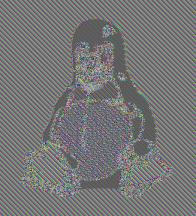
\includegraphics[width=0.3\textwidth]{tux_ecb.jpeg}
  \subfigure{\label{fig:ecbpictc}}
  
\includegraphics[width=0.3\textwidth]{noise.png}
  \caption{a) A picture encrypted in b) ECB-mode and in c) other
    modes, causing an unrevealing pseudo random pattern.}
  \label{fig:ecbpict}
\end{figure}

When encrypting a plaintext with a length over 128 bits, the most
straightforward way is to split the plaintext into 128-bit blocks and
encrypt them individually. This is called the electronic codebook mode
of operation, or ECB. As the blocks can be encrypted and decrypted
independently, this method allows pipelining with unrolled
$Round$s. However, as the AES-algorithm deterministicly yields the
same output given the same input (key and data), it allows an attacker
to guess the ciphertext by trial-and-error. Figure~\ref{fig:ecbpict}
illustrates how ECB reveals data-patterns from the plaintext.

The output feedback (OFB) mode of operation, described in
figure~\ref{fig:ofb}, while not suffering from the same weakness as
the ECB mode, does not benefit from unrolling, as the preceeding
ciphertext is needed to encrypt the current plaintext. The OFB mode
generates a pseudo random (but unguessable, not given the key) string
that is XORed with the plaintext to encrypt, similar to the Vernam
one-time-pad cipher \cite{vernam}.

The only mode of operation considered secure, to my knowledge, that
benefit from loop unrolling, is the counter (CTR) mode. In this mode,
similar to the OFB mode, a pseudorandom string is generated simpy by
encrypting an integer, $i$, corresponding to the current block number, that
is $c_i \leftarrow m_i \oplus E_k(i)$, and similarily $m_i \leftarrow
c_i \oplus E_k(i)$. Whithout feedback, the CTR mode allows random
access during encryption and decryption (for e.g. full disk
encryption), and blocks can be processed in paralell.

\subsection{Decryption and other keysizes}

While this project does not cover decryption and the larger keysizes,
that is 192 and 256 bit, I will shortly outline how this can be
implemented, and roughly estimate the impact on area and performance
it will inflict.

The decryption is rougly the algorithms performed inversely with
reverse operations for $SubBytes$, $ShiftRows$, $MixColumns$ and
$AddKey$. $SubBytes^{-1}$, implemented combinationally, is the same
operation as $SubBytes$, except for the relativily short linear
transform and multiplexers choosing the inverse or normal
transformations. $ShiftRows^{-1}$ has, like $ShiftRows$, the simplest
implementation as wires. $MixColumns^{-1}$ uses different and larger
coefficients than $MixColumns$, demanding 2 more partial products to
be calculated in the galois field multiplications, and thereby causing
longer delays. The calculation of the partial products can be shared
between $MixColumns$ and its inverses. For $AddRoundKey^{-1}$, the
same hardware can be used as in $AddRoundKey$. The keyschedule for the
decryption is the same as for encryption.

Expanding the algorithm to key sizes of 192 and 256 bit requires
changes to the control logic, and the key schedule as well as to the
mere sizes of the key registers. The control logic must be changed as
128, 192, and 256 bit keys respectivily requires 10, 12, and 14
$Round$s to be performed. The key schedule also demands an extension
of the control logic to support the larger key sizes.

Implementing decryption alongside with encryption will, as discussed
above, have negative effect on the performance, as there will be a
greater control overhead. The area will also increase, but as most of
the operations can be generalized to also work in inverse, the area
overhead should not be dramatic. Expansion of the supported key sizes,
in addition to the obvious demand of larger registers, only requires
minor expansion of the control logic.


